% Options for packages loaded elsewhere
\PassOptionsToPackage{unicode}{hyperref}
\PassOptionsToPackage{hyphens}{url}
%
\documentclass[
]{book}
\usepackage{lmodern}
\usepackage{amssymb,amsmath}
\usepackage{ifxetex,ifluatex}
\ifnum 0\ifxetex 1\fi\ifluatex 1\fi=0 % if pdftex
  \usepackage[T1]{fontenc}
  \usepackage[utf8]{inputenc}
  \usepackage{textcomp} % provide euro and other symbols
\else % if luatex or xetex
  \usepackage{unicode-math}
  \defaultfontfeatures{Scale=MatchLowercase}
  \defaultfontfeatures[\rmfamily]{Ligatures=TeX,Scale=1}
\fi
% Use upquote if available, for straight quotes in verbatim environments
\IfFileExists{upquote.sty}{\usepackage{upquote}}{}
\IfFileExists{microtype.sty}{% use microtype if available
  \usepackage[]{microtype}
  \UseMicrotypeSet[protrusion]{basicmath} % disable protrusion for tt fonts
}{}
\makeatletter
\@ifundefined{KOMAClassName}{% if non-KOMA class
  \IfFileExists{parskip.sty}{%
    \usepackage{parskip}
  }{% else
    \setlength{\parindent}{0pt}
    \setlength{\parskip}{6pt plus 2pt minus 1pt}}
}{% if KOMA class
  \KOMAoptions{parskip=half}}
\makeatother
\usepackage{xcolor}
\IfFileExists{xurl.sty}{\usepackage{xurl}}{} % add URL line breaks if available
\IfFileExists{bookmark.sty}{\usepackage{bookmark}}{\usepackage{hyperref}}
\hypersetup{
  pdftitle={Design and Analysis of Experiments with R},
  pdfauthor={D. L. Burrell},
  hidelinks,
  pdfcreator={LaTeX via pandoc}}
\urlstyle{same} % disable monospaced font for URLs
\usepackage{color}
\usepackage{fancyvrb}
\newcommand{\VerbBar}{|}
\newcommand{\VERB}{\Verb[commandchars=\\\{\}]}
\DefineVerbatimEnvironment{Highlighting}{Verbatim}{commandchars=\\\{\}}
% Add ',fontsize=\small' for more characters per line
\usepackage{framed}
\definecolor{shadecolor}{RGB}{248,248,248}
\newenvironment{Shaded}{\begin{snugshade}}{\end{snugshade}}
\newcommand{\AlertTok}[1]{\textcolor[rgb]{0.94,0.16,0.16}{#1}}
\newcommand{\AnnotationTok}[1]{\textcolor[rgb]{0.56,0.35,0.01}{\textbf{\textit{#1}}}}
\newcommand{\AttributeTok}[1]{\textcolor[rgb]{0.77,0.63,0.00}{#1}}
\newcommand{\BaseNTok}[1]{\textcolor[rgb]{0.00,0.00,0.81}{#1}}
\newcommand{\BuiltInTok}[1]{#1}
\newcommand{\CharTok}[1]{\textcolor[rgb]{0.31,0.60,0.02}{#1}}
\newcommand{\CommentTok}[1]{\textcolor[rgb]{0.56,0.35,0.01}{\textit{#1}}}
\newcommand{\CommentVarTok}[1]{\textcolor[rgb]{0.56,0.35,0.01}{\textbf{\textit{#1}}}}
\newcommand{\ConstantTok}[1]{\textcolor[rgb]{0.00,0.00,0.00}{#1}}
\newcommand{\ControlFlowTok}[1]{\textcolor[rgb]{0.13,0.29,0.53}{\textbf{#1}}}
\newcommand{\DataTypeTok}[1]{\textcolor[rgb]{0.13,0.29,0.53}{#1}}
\newcommand{\DecValTok}[1]{\textcolor[rgb]{0.00,0.00,0.81}{#1}}
\newcommand{\DocumentationTok}[1]{\textcolor[rgb]{0.56,0.35,0.01}{\textbf{\textit{#1}}}}
\newcommand{\ErrorTok}[1]{\textcolor[rgb]{0.64,0.00,0.00}{\textbf{#1}}}
\newcommand{\ExtensionTok}[1]{#1}
\newcommand{\FloatTok}[1]{\textcolor[rgb]{0.00,0.00,0.81}{#1}}
\newcommand{\FunctionTok}[1]{\textcolor[rgb]{0.00,0.00,0.00}{#1}}
\newcommand{\ImportTok}[1]{#1}
\newcommand{\InformationTok}[1]{\textcolor[rgb]{0.56,0.35,0.01}{\textbf{\textit{#1}}}}
\newcommand{\KeywordTok}[1]{\textcolor[rgb]{0.13,0.29,0.53}{\textbf{#1}}}
\newcommand{\NormalTok}[1]{#1}
\newcommand{\OperatorTok}[1]{\textcolor[rgb]{0.81,0.36,0.00}{\textbf{#1}}}
\newcommand{\OtherTok}[1]{\textcolor[rgb]{0.56,0.35,0.01}{#1}}
\newcommand{\PreprocessorTok}[1]{\textcolor[rgb]{0.56,0.35,0.01}{\textit{#1}}}
\newcommand{\RegionMarkerTok}[1]{#1}
\newcommand{\SpecialCharTok}[1]{\textcolor[rgb]{0.00,0.00,0.00}{#1}}
\newcommand{\SpecialStringTok}[1]{\textcolor[rgb]{0.31,0.60,0.02}{#1}}
\newcommand{\StringTok}[1]{\textcolor[rgb]{0.31,0.60,0.02}{#1}}
\newcommand{\VariableTok}[1]{\textcolor[rgb]{0.00,0.00,0.00}{#1}}
\newcommand{\VerbatimStringTok}[1]{\textcolor[rgb]{0.31,0.60,0.02}{#1}}
\newcommand{\WarningTok}[1]{\textcolor[rgb]{0.56,0.35,0.01}{\textbf{\textit{#1}}}}
\usepackage{longtable,booktabs}
% Correct order of tables after \paragraph or \subparagraph
\usepackage{etoolbox}
\makeatletter
\patchcmd\longtable{\par}{\if@noskipsec\mbox{}\fi\par}{}{}
\makeatother
% Allow footnotes in longtable head/foot
\IfFileExists{footnotehyper.sty}{\usepackage{footnotehyper}}{\usepackage{footnote}}
\makesavenoteenv{longtable}
\usepackage{graphicx,grffile}
\makeatletter
\def\maxwidth{\ifdim\Gin@nat@width>\linewidth\linewidth\else\Gin@nat@width\fi}
\def\maxheight{\ifdim\Gin@nat@height>\textheight\textheight\else\Gin@nat@height\fi}
\makeatother
% Scale images if necessary, so that they will not overflow the page
% margins by default, and it is still possible to overwrite the defaults
% using explicit options in \includegraphics[width, height, ...]{}
\setkeys{Gin}{width=\maxwidth,height=\maxheight,keepaspectratio}
% Set default figure placement to htbp
\makeatletter
\def\fps@figure{htbp}
\makeatother
\setlength{\emergencystretch}{3em} % prevent overfull lines
\providecommand{\tightlist}{%
  \setlength{\itemsep}{0pt}\setlength{\parskip}{0pt}}
\setcounter{secnumdepth}{5}
\usepackage{booktabs}
\usepackage[]{natbib}
\bibliographystyle{apalike}

\title{Design and Analysis of Experiments with R}
\usepackage{etoolbox}
\makeatletter
\providecommand{\subtitle}[1]{% add subtitle to \maketitle
  \apptocmd{\@title}{\par {\large #1 \par}}{}{}
}
\makeatother
\subtitle{A Modern Approach}
\author{D. L. Burrell}
\date{2021-07-08}

\begin{document}
\maketitle

{
\setcounter{tocdepth}{1}
\tableofcontents
}
\hypertarget{prerequisites}{%
\chapter{Prerequisites}\label{prerequisites}}

\hypertarget{intro}{%
\chapter{Introduction}\label{intro}}

You can label chapter and section titles using \texttt{\{\#label\}} after them, e.g., we can reference Chapter \ref{intro}. If you do not manually label them, there will be automatic labels anyway, e.g., Chapter \ref{methods}.

Figures and tables with captions will be placed in \texttt{figure} and \texttt{table} environments, respectively.

\begin{Shaded}
\begin{Highlighting}[]
\KeywordTok{par}\NormalTok{(}\DataTypeTok{mar =} \KeywordTok{c}\NormalTok{(}\DecValTok{4}\NormalTok{, }\DecValTok{4}\NormalTok{, }\FloatTok{.1}\NormalTok{, }\FloatTok{.1}\NormalTok{))}
\KeywordTok{plot}\NormalTok{(pressure, }\DataTypeTok{type =} \StringTok{'b'}\NormalTok{, }\DataTypeTok{pch =} \DecValTok{19}\NormalTok{)}
\end{Highlighting}
\end{Shaded}

\begin{figure}

{\centering 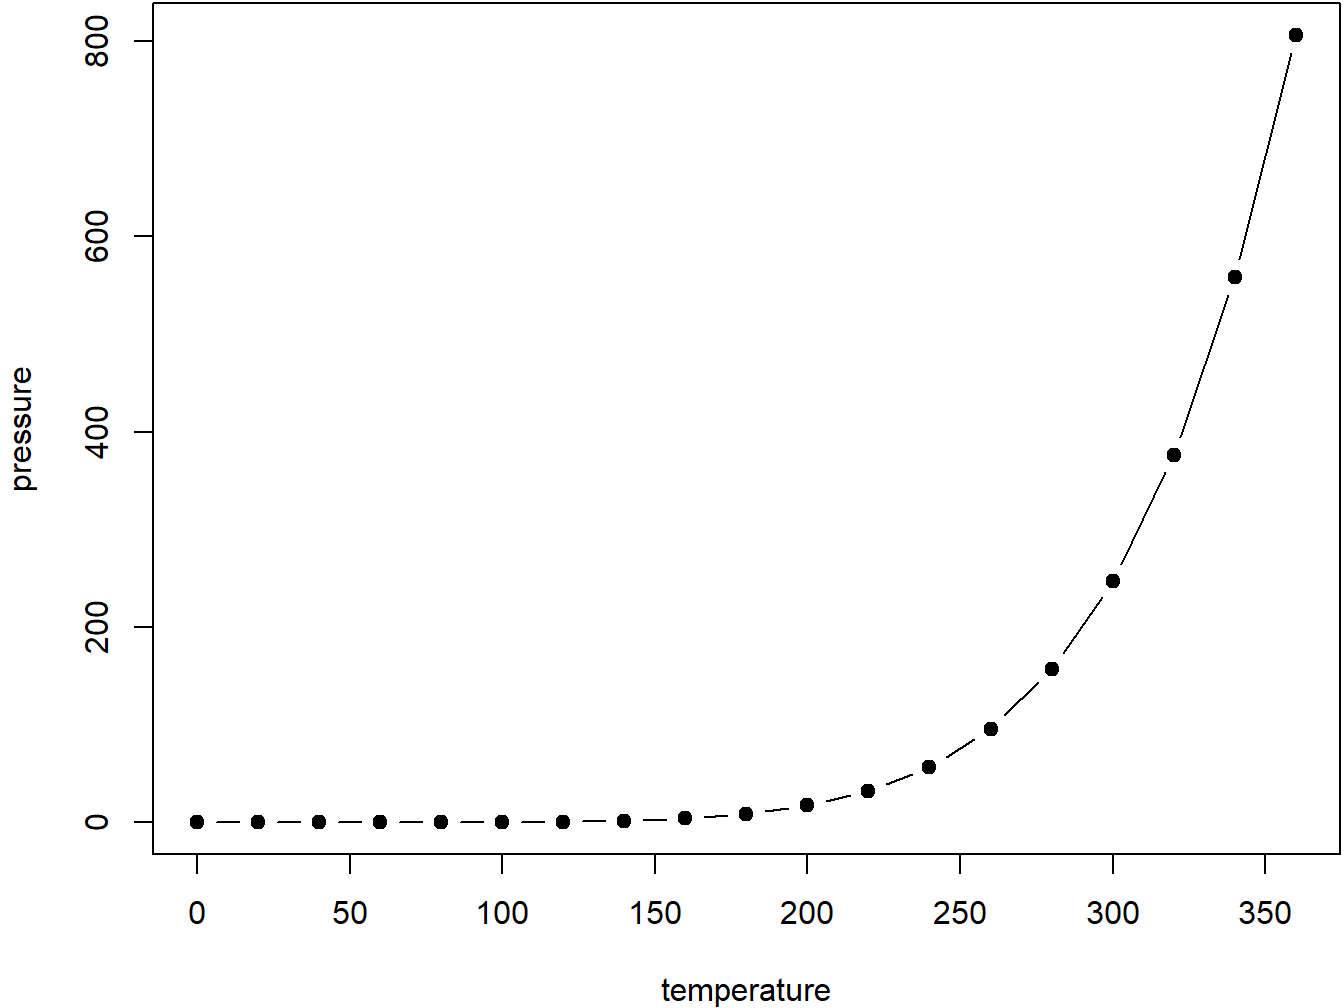
\includegraphics[width=0.8\linewidth]{STA3300_bookdown_files/figure-latex/nice-fig-1} 

}

\caption{Here is a nice figure!}\label{fig:nice-fig}
\end{figure}

Reference a figure by its code chunk label with the \texttt{fig:} prefix, e.g., see Figure \ref{fig:nice-fig}. Similarly, you can reference tables generated from \texttt{knitr::kable()}, e.g., see Table \ref{tab:nice-tab}.

\begin{Shaded}
\begin{Highlighting}[]
\NormalTok{knitr}\OperatorTok{::}\KeywordTok{kable}\NormalTok{(}
  \KeywordTok{head}\NormalTok{(iris, }\DecValTok{20}\NormalTok{), }\DataTypeTok{caption =} \StringTok{'Here is a nice table!'}\NormalTok{,}
  \DataTypeTok{booktabs =} \OtherTok{TRUE}
\NormalTok{)}
\end{Highlighting}
\end{Shaded}

\begin{table}

\caption{\label{tab:nice-tab}Here is a nice table!}
\centering
\begin{tabular}[t]{rrrrl}
\toprule
Sepal.Length & Sepal.Width & Petal.Length & Petal.Width & Species\\
\midrule
5.1 & 3.5 & 1.4 & 0.2 & setosa\\
4.9 & 3.0 & 1.4 & 0.2 & setosa\\
4.7 & 3.2 & 1.3 & 0.2 & setosa\\
4.6 & 3.1 & 1.5 & 0.2 & setosa\\
5.0 & 3.6 & 1.4 & 0.2 & setosa\\
\addlinespace
5.4 & 3.9 & 1.7 & 0.4 & setosa\\
4.6 & 3.4 & 1.4 & 0.3 & setosa\\
5.0 & 3.4 & 1.5 & 0.2 & setosa\\
4.4 & 2.9 & 1.4 & 0.2 & setosa\\
4.9 & 3.1 & 1.5 & 0.1 & setosa\\
\addlinespace
5.4 & 3.7 & 1.5 & 0.2 & setosa\\
4.8 & 3.4 & 1.6 & 0.2 & setosa\\
4.8 & 3.0 & 1.4 & 0.1 & setosa\\
4.3 & 3.0 & 1.1 & 0.1 & setosa\\
5.8 & 4.0 & 1.2 & 0.2 & setosa\\
\addlinespace
5.7 & 4.4 & 1.5 & 0.4 & setosa\\
5.4 & 3.9 & 1.3 & 0.4 & setosa\\
5.1 & 3.5 & 1.4 & 0.3 & setosa\\
5.7 & 3.8 & 1.7 & 0.3 & setosa\\
5.1 & 3.8 & 1.5 & 0.3 & setosa\\
\bottomrule
\end{tabular}
\end{table}

You can write citations, too. For example, we are using the \textbf{bookdown} package \citep{R-bookdown} in this sample book, which was built on top of R Markdown and \textbf{knitr} \citep{xie2015}.

\hypertarget{literature}{%
\chapter{Literature}\label{literature}}

Here is a review of existing methods.

\hypertarget{statistical-models}{%
\chapter{Statistical Models}\label{statistical-models}}

One of the great scientific achievements humanity has made is the ability to conceptualize complex phenomena and processes in the natural world through models that amplify the pertinent facts and relationships of interest and provide a logical platform from which to study systems that drive decision-making. Most scientific models can be expressed as mathematical abstractions. Two broad classes of mathematical models are \textbf{deterministic models} and \textbf{stochastic models}. Broadly speaking, deterministic models leave nothing to chance and blatantly ignore uncertainties. For example the concentration \(c\) of a pollutant in a river at a point \(x\) and time \(t\) can be modeled as:
\[
c(x,t)=c_0 (x-vt)e^{-kt},
\]
where \(c_0(x)\) is the initial pollutant concentration at point \(x\), \(v\) is the water velocity, and \(k\) is a proportionality constant, measuring the efficiency of bacterial decomposition of the pollutant. This is a deterministic model: given inputs \(x, v\) and \(c_0\), the pollutant concentration at location \(x\) and time \(t\) is predicted with certainty. Such a model makes a very strong assumption that the model is correct and the inputs are measured with perfect precision and accuracy. But the pollutant concentration makes certain assumptions: (i) that the pollutant concentration is uniform in all directions except downstream flow, (ii) there are no diffusive effects due to to contour irregularities and turbulence, (iii) the pollutant decays as a negative exponential due to bacterial action, (iv) the bacterial efficiency is time-homogeneous, and (v) there is thorough mixing of the pollutant in the water. These assumptions are reasonable, but they not necessarily (always) true. The uncertainty of the effects at a particular location along the river and point in time can be incorporated by casting the model stochastically:
\[
c(x,t) = c_0 (x-vt)e^{-kt} + e
\]
where \(e \sim D(0,\sigma^2)\), for some probability distribution \(D\). Allowing for the random deviation \(e\) we are now claiming that \(c(x,t)\) is a random variable with expectation:
\[
\mathbb E[c(x,t)] = c_0 (x-vt)e^{-kt} 
\]

\hypertarget{linear-models-in-r}{%
\section{Linear Models in R}\label{linear-models-in-r}}

Most R functions uses a formula representation to represent regression models (for continuous variables) or means and effects models (for categorical variables):

\begin{Shaded}
\begin{Highlighting}[]
\NormalTok{response }\OperatorTok{~}\StringTok{ }\NormalTok{model}
\end{Highlighting}
\end{Shaded}

where the tilde (\textasciitilde) defines a model formula and \texttt{model} represents a set of terms to include as predictors in the model. Terms are included by their variable names and various operators such as \texttt{+} (include in model), \texttt{-} (exclude from model), \texttt{:} (interaction), \texttt{*} (full factorial structure), and so on. The intercept term (which can be explicitly denoted in a model as a \texttt{1}) is implicitly defined and need not be specified (although I often do for completeness). Thus the following model formulae are equivalent (all include the intercept):

\begin{Shaded}
\begin{Highlighting}[]
\NormalTok{Y }\OperatorTok{~}\StringTok{ }\NormalTok{X}
\NormalTok{Y }\OperatorTok{~}\StringTok{ }\DecValTok{1} \OperatorTok{+}\StringTok{ }\NormalTok{X}
\NormalTok{Y }\OperatorTok{~}\StringTok{ }\NormalTok{X }\OperatorTok{+}\StringTok{ }\DecValTok{1}
\end{Highlighting}
\end{Shaded}

whereas these formulae express different ways of excluding the intercept:

\begin{Shaded}
\begin{Highlighting}[]
\NormalTok{Y }\OperatorTok{~}\StringTok{ }\DecValTok{-1} \OperatorTok{+}\StringTok{ }\NormalTok{X}
\NormalTok{Y }\OperatorTok{~}\StringTok{ }\NormalTok{X }\OperatorTok{-}\StringTok{ }\DecValTok{1}
\end{Highlighting}
\end{Shaded}

Linear models are fitted using the method of ordinary least squares by providing the model formula as an argument to the \texttt{lm()} function. For example, we could generate a fictitious response variable (\texttt{Y}) and a fictitious continuous predictor (\texttt{X}) as follows:

\begin{Shaded}
\begin{Highlighting}[]
\CommentTok{# Load packages}
\ControlFlowTok{if}\NormalTok{(}\OperatorTok{!}\KeywordTok{require}\NormalTok{(pacman)) }\KeywordTok{install.packages}\NormalTok{(}\StringTok{"pacman"}\NormalTok{)}
\end{Highlighting}
\end{Shaded}

\begin{verbatim}
## Loading required package: pacman
\end{verbatim}

\begin{Shaded}
\begin{Highlighting}[]
\KeywordTok{library}\NormalTok{(pacman)}
\KeywordTok{p_load}\NormalTok{(tidyverse)}

\CommentTok{# Generate data set}
\NormalTok{N =}\StringTok{ }\DecValTok{10}
\NormalTok{fictitious_data =}\StringTok{ }\KeywordTok{tibble}\NormalTok{(}
   \DataTypeTok{X =} \DecValTok{1}\OperatorTok{:}\NormalTok{N,}
   \DataTypeTok{Y =} \FloatTok{0.9}\OperatorTok{*}\NormalTok{X }\OperatorTok{+}\StringTok{ }\KeywordTok{rnorm}\NormalTok{(}\DataTypeTok{n=}\NormalTok{N, }\DataTypeTok{mean=}\DecValTok{0}\NormalTok{, }\DataTypeTok{sd=}\FloatTok{0.5}\NormalTok{)}
\NormalTok{)}

\CommentTok{# Plot data}
\KeywordTok{ggplot}\NormalTok{(}\DataTypeTok{data =}\NormalTok{ fictitious_data,}
       \DataTypeTok{mapping =} \KeywordTok{aes}\NormalTok{(}\DataTypeTok{x=}\NormalTok{X, }\DataTypeTok{y=}\NormalTok{Y)) }\OperatorTok{+}
\StringTok{   }\KeywordTok{geom_point}\NormalTok{(}\DataTypeTok{colour =} \StringTok{"blue"}\NormalTok{) }\OperatorTok{+}
\StringTok{   }\KeywordTok{geom_smooth}\NormalTok{(}\DataTypeTok{method =} \StringTok{"lm"}\NormalTok{,}
               \DataTypeTok{formula =}\NormalTok{ y }\OperatorTok{~}\StringTok{ }\NormalTok{x,}
               \DataTypeTok{se =} \OtherTok{FALSE}\NormalTok{,}
               \DataTypeTok{colour =} \StringTok{"darkgreen"}\NormalTok{) }\OperatorTok{+}
\StringTok{   }\KeywordTok{theme_classic}\NormalTok{()}
\end{Highlighting}
\end{Shaded}

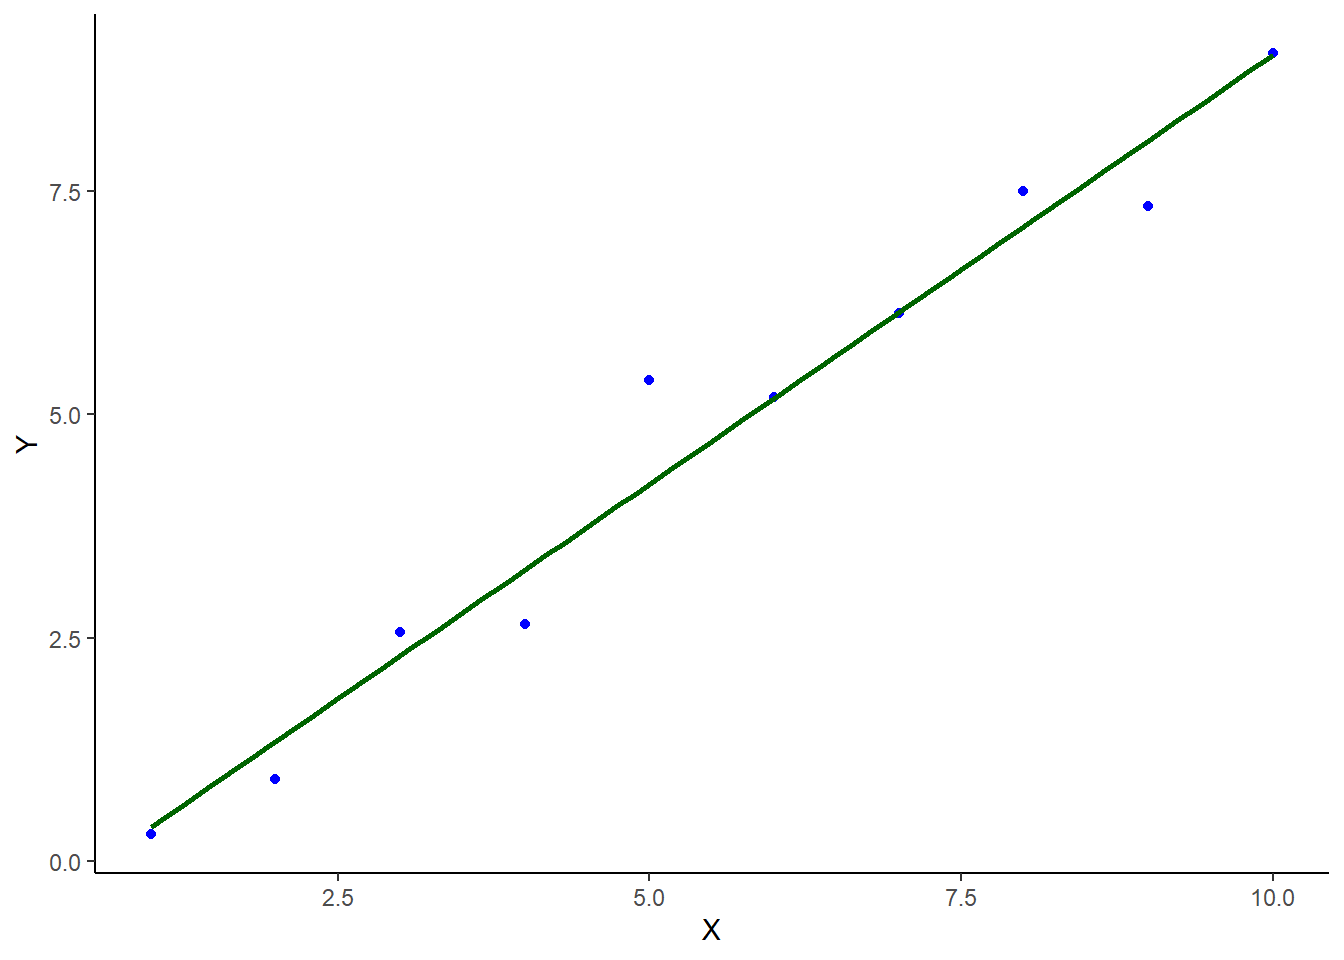
\includegraphics{STA3300_bookdown_files/figure-latex/unnamed-chunk-5-1.pdf}
The plot shows the data points and a simple linear regression line fit through them. To fit the regression in such a way as to be able to work with the estimated parameters we use \texttt{lm()}:

\begin{Shaded}
\begin{Highlighting}[]
\CommentTok{# Fit simple linear regression model}
\NormalTok{fictitious_lm =}\StringTok{ }\KeywordTok{lm}\NormalTok{(}
   \DataTypeTok{formula =}\NormalTok{ Y }\OperatorTok{~}\StringTok{ }\DecValTok{1} \OperatorTok{+}\StringTok{ }\NormalTok{X,}
   \DataTypeTok{data =}\NormalTok{ fictitious_data)}
\end{Highlighting}
\end{Shaded}

To examine the estimated parameters (and hypothesis tests) from the fitted model we can use the function \texttt{summary()}:

\begin{Shaded}
\begin{Highlighting}[]
\CommentTok{# Summary of regression }
\KeywordTok{summary}\NormalTok{(fictitious_lm)}
\end{Highlighting}
\end{Shaded}

\begin{verbatim}
## 
## Call:
## lm(formula = Y ~ 1 + X, data = fictitious_data)
## 
## Residuals:
##      Min       1Q   Median       3Q      Max 
## -0.72350 -0.05239  0.06048  0.19485  0.58455 
## 
## Coefficients:
##             Estimate Std. Error t value Pr(>|t|)    
## (Intercept) -0.12273    0.27348  -0.449    0.666    
## X            0.92416    0.04408  20.968 2.81e-08 ***
## ---
## Signif. codes:  0 '***' 0.001 '**' 0.01 '*' 0.05 '.' 0.1 ' ' 1
## 
## Residual standard error: 0.4003 on 8 degrees of freedom
## Multiple R-squared:  0.9821, Adjusted R-squared:  0.9799 
## F-statistic: 439.6 on 1 and 8 DF,  p-value: 2.809e-08
\end{verbatim}

There is a lot of useful information presented here, however it is not necessarily easy to access and work with in successive computations. This is where the \texttt{broom} package comes in. There are three main functions that allow us to extract pertinent information and store it in data frames, for easy access later. The functions are:

\begin{itemize}
\tightlist
\item
  \texttt{tidy()}: returns the statistical findings of the model (such as coefficients)
\item
  \texttt{glance()}: returns a concise one-row summary of the model
\item
  `\texttt{augment()}: adds prediction columns to the data being modeled
\end{itemize}

Using \texttt{tidy(fictitious\_lm)} we can extract the pertitent statistical information such as estimates, standard errors, test statistics and p-values:

\begin{Shaded}
\begin{Highlighting}[]
\CommentTok{# Ensure broom package is loaded}
\KeywordTok{p_load}\NormalTok{(broom)}

\CommentTok{# Set output digits to 3 for printing}
\KeywordTok{options}\NormalTok{(}\DataTypeTok{digits=}\DecValTok{3}\NormalTok{)}

\CommentTok{# tidy() output}
\KeywordTok{tidy}\NormalTok{(}\DataTypeTok{x =}\NormalTok{ fictitious_lm,}
     \DataTypeTok{conf.int =} \OtherTok{TRUE}\NormalTok{,}
     \DataTypeTok{conf.level =} \FloatTok{0.95}\NormalTok{)}
\end{Highlighting}
\end{Shaded}

\begin{verbatim}
## # A tibble: 2 x 7
##   term        estimate std.error statistic      p.value conf.low conf.high
##   <chr>          <dbl>     <dbl>     <dbl>        <dbl>    <dbl>     <dbl>
## 1 (Intercept)   -0.123    0.273     -0.449 0.666          -0.753     0.508
## 2 X              0.924    0.0441    21.0   0.0000000281    0.823     1.03
\end{verbatim}

From this we see, for example, that the simple linear regression equation is given by:
\[
\hat Y_i = 0.387 + 0.871\times X_i,  
\]
and that we cannot reject \(H_0: \beta_0=0\) (p = 0.334), but we strongly reject \(H_0:\beta_1 = 0\) (p = 0.000000536), indicating that a model with no zero intercept will be just as good:

\begin{Shaded}
\begin{Highlighting}[]
\NormalTok{fictitious_lm}\FloatTok{.2}\NormalTok{ =}\StringTok{ }\KeywordTok{lm}\NormalTok{(}
   \DataTypeTok{formula =}\NormalTok{ Y }\OperatorTok{~}\StringTok{ }\DecValTok{-1} \OperatorTok{+}\StringTok{ }\NormalTok{X,}
   \DataTypeTok{data =}\NormalTok{ fictitious_data)}

\CommentTok{# Compare the full model to the reduced model with zero intercept}
\KeywordTok{anova}\NormalTok{(fictitious_lm, fictitious_lm}\FloatTok{.2}\NormalTok{) }\OperatorTok\StringTok{ }\KeywordTok{tidy}\NormalTok{()}
\end{Highlighting}
\end{Shaded}

\begin{verbatim}
## # A tibble: 2 x 6
##   res.df   rss    df   sumsq statistic p.value
##    <dbl> <dbl> <dbl>   <dbl>     <dbl>   <dbl>
## 1      8  1.28    NA NA         NA      NA    
## 2      9  1.31    -1 -0.0323     0.201   0.666
\end{verbatim}

We see that there is no significant reduction in sums of squares between the model with the unconstrained intercept and the model with the intercept constrained to be zero. We therefore opt to use the latter model:

\begin{Shaded}
\begin{Highlighting}[]
\KeywordTok{tidy}\NormalTok{(}\DataTypeTok{x =}\NormalTok{ fictitious_lm}\FloatTok{.2}\NormalTok{,}
     \DataTypeTok{conf.int =} \OtherTok{TRUE}\NormalTok{,}
     \DataTypeTok{conf.level =} \FloatTok{0.95}\NormalTok{)}
\end{Highlighting}
\end{Shaded}

\begin{verbatim}
## # A tibble: 1 x 7
##   term  estimate std.error statistic  p.value conf.low conf.high
##   <chr>    <dbl>     <dbl>     <dbl>    <dbl>    <dbl>     <dbl>
## 1 X        0.907    0.0195      46.5 4.88e-12    0.863     0.951
\end{verbatim}

which has regression equation:
\[
\hat Y_i=0.927\times X_i
\]

Using \texttt{glance(fictitious\_lm.2)} we can obtain a one-row summary of the reduced model. For the linear model this summary contains various statistics about the fit of the model, such as the residual standard error and \(R^2\):

\begin{Shaded}
\begin{Highlighting}[]
\CommentTok{# One-row summary at a glance}
\KeywordTok{glance}\NormalTok{(}\DataTypeTok{x =}\NormalTok{ fictitious_lm}\FloatTok{.2}\NormalTok{)}
\end{Highlighting}
\end{Shaded}

\begin{verbatim}
## # A tibble: 1 x 12
##   r.squared adj.r.squared sigma statistic p.value    df logLik   AIC   BIC
##       <dbl>         <dbl> <dbl>     <dbl>   <dbl> <dbl>  <dbl> <dbl> <dbl>
## 1     0.996         0.995 0.382        NA      NA    NA  -4.04  12.1  12.7
## # ... with 3 more variables: deviance <dbl>, df.residual <int>, nobs <int>
\end{verbatim}

Using \texttt{augment(fictitious\_lm.2)} we get back an observation-level data frame containing the original data used to fit the model as well as fitted values (\texttt{.fitted}) and standard errors (\texttt{.se.fit}).

\begin{Shaded}
\begin{Highlighting}[]
\KeywordTok{augment}\NormalTok{(}\DataTypeTok{x =}\NormalTok{ fictitious_lm}\FloatTok{.2}\NormalTok{,}
        \DataTypeTok{newdata =} \OtherTok{NULL}\NormalTok{,}
        \DataTypeTok{se_fit =} \OtherTok{TRUE}\NormalTok{,}
        \DataTypeTok{interval =} \StringTok{"none"}\NormalTok{) }\CommentTok{# confidence, prediction}
\end{Highlighting}
\end{Shaded}

\begin{verbatim}
## # A tibble: 10 x 9
##        Y     X .fitted .se.fit  .resid    .hat .sigma  .cooksd .std.resid
##    <dbl> <int>   <dbl>   <dbl>   <dbl>   <dbl>  <dbl>    <dbl>      <dbl>
##  1 0.829     1   0.907  0.0195 -0.0773 0.00260  0.404 0.000107    -0.202 
##  2 1.20      2   1.81   0.0390 -0.610  0.0104   0.343 0.0270      -1.60  
##  3 2.90      3   2.72   0.0584  0.176  0.0234   0.400 0.00519      0.466 
##  4 3.56      4   3.63   0.0779 -0.0659 0.0416   0.405 0.00135     -0.176 
##  5 4.67      5   4.53   0.0974  0.134  0.0649   0.402 0.00917      0.363 
##  6 6.01      6   5.44   0.117   0.567  0.0935   0.346 0.251        1.56  
##  7 6.55      7   6.35   0.136   0.203  0.127    0.398 0.0473       0.570 
##  8 6.55      8   7.25   0.156  -0.706  0.166    0.299 0.816       -2.02  
##  9 8.13      9   8.16   0.175  -0.0303 0.210    0.405 0.00213     -0.0894
## 10 9.21     10   9.07   0.195   0.146  0.260    0.401 0.0689       0.443
\end{verbatim}

Notice that \texttt{augment()} also appends model-specific statistics that enable deeper exploration of the fit of the model. For example, we can explore how well the model fits by plotting the observed values \texttt{Y} against the fitted values \texttt{.fitted} (compare this to the plot constructed earlier, which was based on the full model with unconstrained intercept).

\begin{Shaded}
\begin{Highlighting}[]
\NormalTok{p1 =}\StringTok{ }\KeywordTok{augment}\NormalTok{(}\DataTypeTok{x =}\NormalTok{ fictitious_lm}\FloatTok{.2}\NormalTok{) }\OperatorTok
\StringTok{   }\KeywordTok{ggplot}\NormalTok{(}\DataTypeTok{mapping =} \KeywordTok{aes}\NormalTok{(}\DataTypeTok{x =}\NormalTok{ X)) }\OperatorTok{+}
\StringTok{   }\KeywordTok{geom_point}\NormalTok{(}\DataTypeTok{mapping =} \KeywordTok{aes}\NormalTok{(}\DataTypeTok{y =}\NormalTok{ Y), }\DataTypeTok{colour=}\StringTok{"blue"}\NormalTok{) }\OperatorTok{+}
\StringTok{   }\KeywordTok{geom_line}\NormalTok{(}\DataTypeTok{mapping =} \KeywordTok{aes}\NormalTok{(}\DataTypeTok{y =}\NormalTok{ .fitted), }\DataTypeTok{colour=}\StringTok{"magenta"}\NormalTok{) }\OperatorTok{+}
\StringTok{   }\KeywordTok{theme_classic}\NormalTok{()}

\NormalTok{p1}
\end{Highlighting}
\end{Shaded}

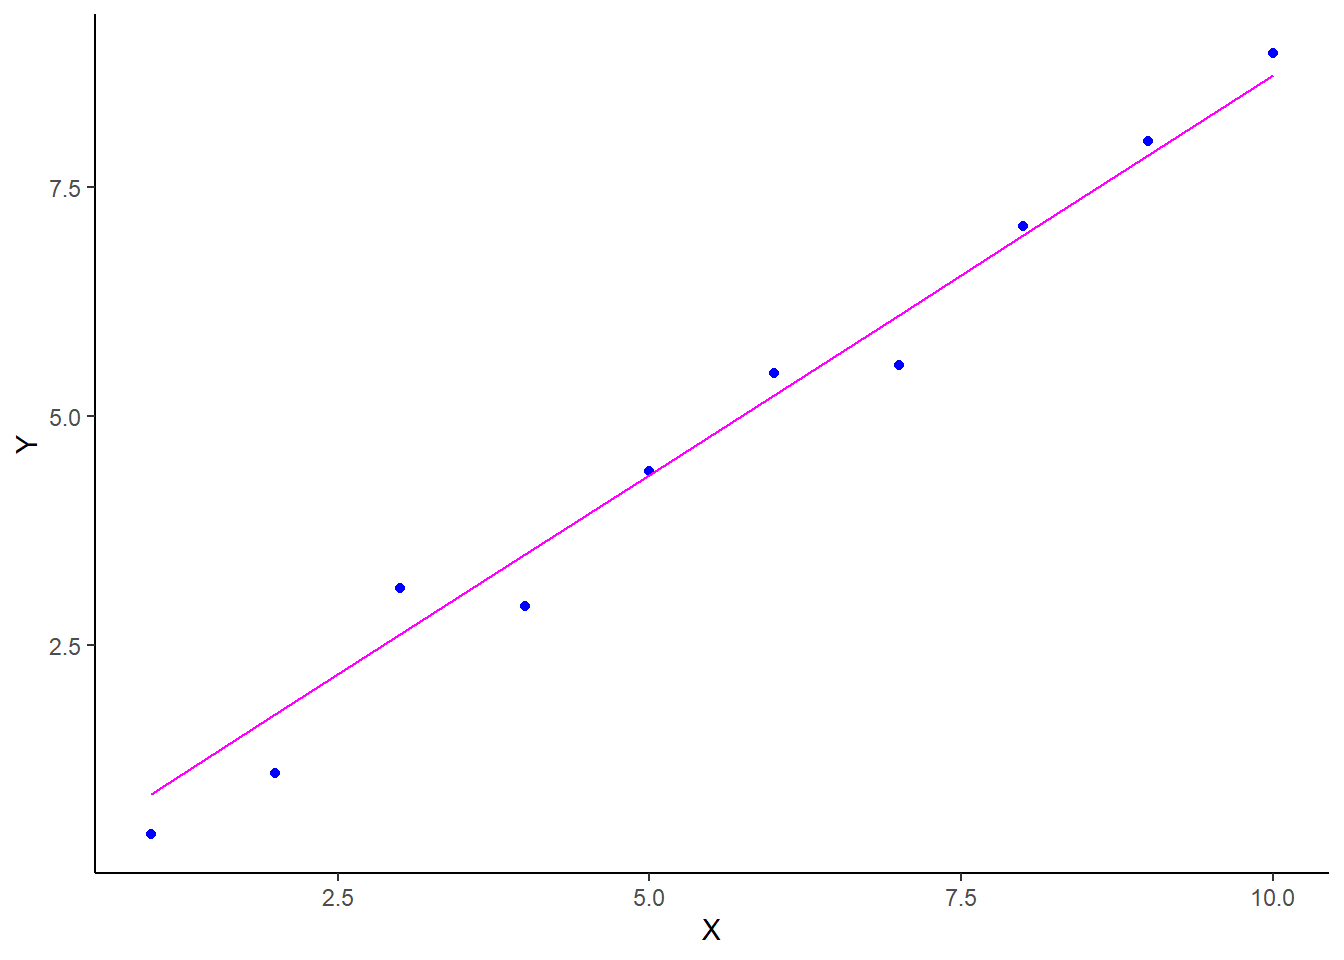
\includegraphics{STA3300_bookdown_files/figure-latex/unnamed-chunk-13-1.pdf}
We could overlay the unconstrained model as follows:

\begin{Shaded}
\begin{Highlighting}[]
\KeywordTok{ggplot}\NormalTok{(}\DataTypeTok{data =}\NormalTok{ fictitious_data,}
       \DataTypeTok{mapping =} \KeywordTok{aes}\NormalTok{(}\DataTypeTok{x=}\NormalTok{X, }\DataTypeTok{y=}\NormalTok{Y)) }\OperatorTok{+}
\StringTok{   }\KeywordTok{geom_point}\NormalTok{(}\DataTypeTok{colour =} \StringTok{"blue"}\NormalTok{) }\OperatorTok{+}
\StringTok{   }\KeywordTok{geom_smooth}\NormalTok{(}\DataTypeTok{method =} \StringTok{"lm"}\NormalTok{,}
               \DataTypeTok{formula =}\NormalTok{ y }\OperatorTok{~}\StringTok{ }\NormalTok{x,}
               \DataTypeTok{se =} \OtherTok{FALSE}\NormalTok{,}
               \DataTypeTok{colour =} \StringTok{"darkgreen"}\NormalTok{) }\OperatorTok{+}
\StringTok{   }\KeywordTok{geom_smooth}\NormalTok{(}\DataTypeTok{method =} \StringTok{"lm"}\NormalTok{,}
               \DataTypeTok{formula =}\NormalTok{ y }\OperatorTok{~}\StringTok{ }\DecValTok{-1} \OperatorTok{+}\StringTok{ }\NormalTok{x,}
               \DataTypeTok{se =} \OtherTok{FALSE}\NormalTok{,}
               \DataTypeTok{colour =} \StringTok{"magenta"}\NormalTok{) }\OperatorTok{+}
\StringTok{   }\KeywordTok{theme_classic}\NormalTok{()}
\end{Highlighting}
\end{Shaded}

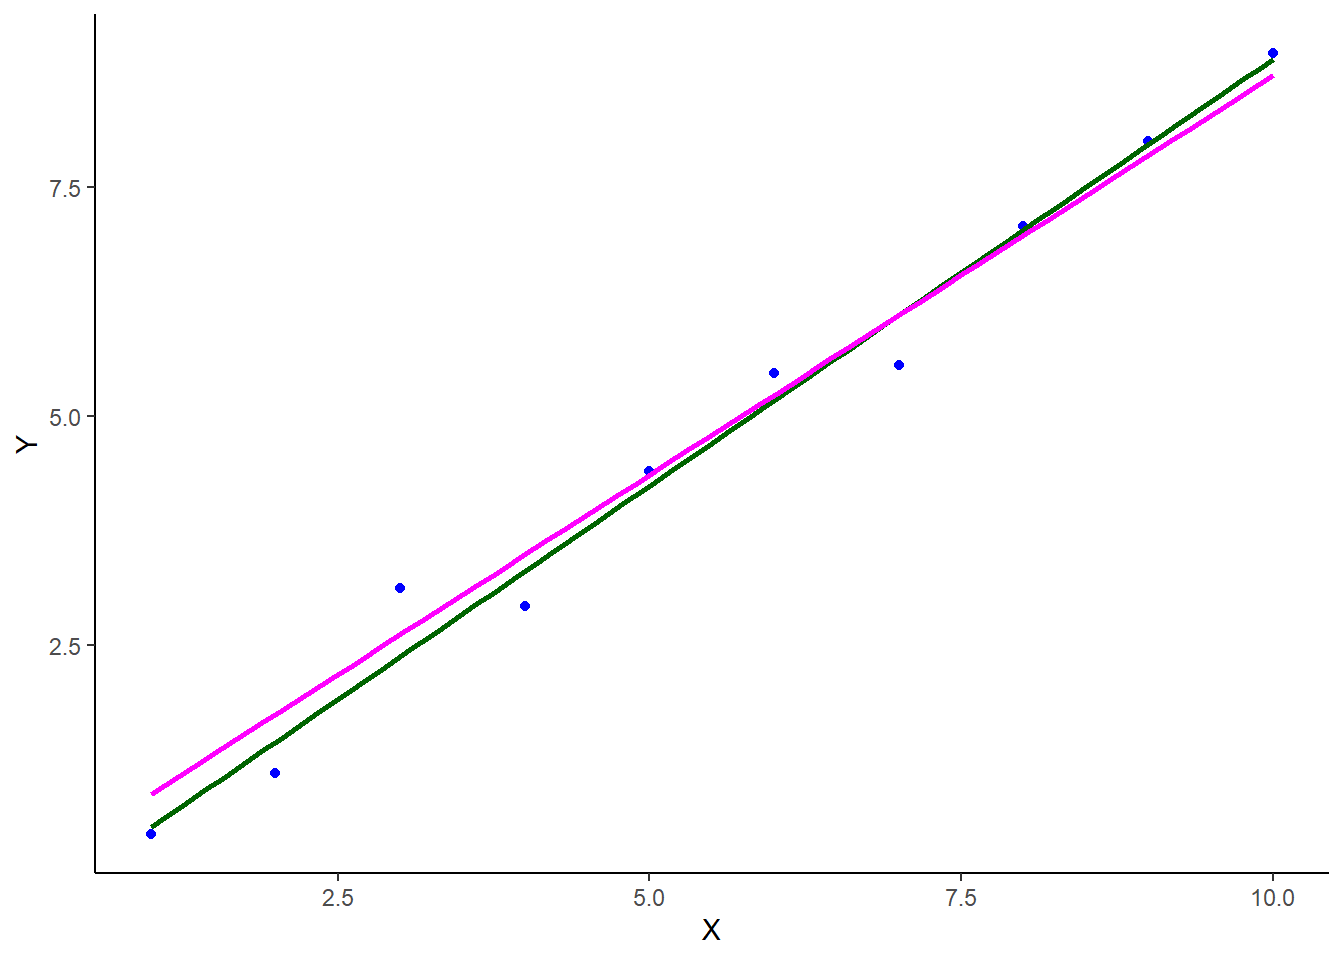
\includegraphics{STA3300_bookdown_files/figure-latex/unnamed-chunk-14-1.pdf}

\hypertarget{estimating-linear-model-parameters}{%
\section{Estimating linear model parameters}\label{estimating-linear-model-parameters}}

During model fitting, parameters can be estimated using a variety of estimation methods. The methods of ordinary least squares (OLS), maximum likelihood (ML) and restricted maximum likelihood (REML) are the most common. The OLS estimates of parameters minimize the sum of squared deviations between the observed and fitted values (a function of the model parameters). There are several variants on the method of ordinary least squares: weighted least squares can accommodate data that varies in quality and generalized least squares can accommodate heterogeneous variances and correlated data. The model we've been looking at is usually referred to as the general linear model (and it was once the most general linear model, but it is not very general by today's standards). Broadly speaking we consider such a model with purely continuous predictor variables to be a \textbf{regression} model, while a model with purely categorical predictors is an \textbf{analysis of variance (ANOVA)} model. Models that incorporate both continuous and categorical predictors are \textbf{analysis of covariance (ANCOVA)} models.

ML estimators estimate model parameters such that the (log) likelihood of obtaining the observed data is maximized. Under standard assumptions (normal data, constant variance, independent observations) the ML estimates are identical to the OLS estimates. However, maximum likelihood parameter estimation extends beyond the general linear model to the so-called ``generalized'' linear model, which are not restricted to normally distributed errors and response. Instead they generalize to any distribution belonging to the family of distribution models called exponential dispersion models (which include normal, binomial, Poisson, gamma, negative binomial and others).

\hypertarget{applications}{%
\chapter{Applications}\label{applications}}

Some \emph{significant} applications are demonstrated in this chapter.

\hypertarget{example-one}{%
\section{Example one}\label{example-one}}

\hypertarget{example-two}{%
\section{Example two}\label{example-two}}

\hypertarget{final-words}{%
\chapter{Final Words}\label{final-words}}

We have finished a nice book.

  \bibliography{book.bib,packages.bib}

\end{document}
